\chapter{Grundlagen}
In diesem Kapitel erkläre ich grundlegende Begriffe, die für das Verständnis der Arbeit unabdingbar sind.

\section{Cloud Computing}
Laut der Definition des National Institute of Standards and Technology (NIST), ist Cloud Computing ein Modell, dass einen einfachen on-demand Zugriff auf eine Menge von EDV Ressourcen ermöglicht, welche schnell und ohne Interaktion eines Service Providers bereitgestellt oder freigegeben werden können\cite{mell_nist_2011}.
Cloud Computing zeichnet sich demnach durch fünf Charakteristiken aus. Diese sind die bedarfsorientierte Bereitstellung von Ressourcen die durch einen Systembenutzer ausgelöst wird, den einfachen Zugriff über heterogene Plattformen hinweg durch standardisierte Netzwerkmechanismen, das Pooling von Servern und die schnelle und automatisierte Skalierung, scheinbar unendlich verfügbare Ressourcen und das dauerhafte Messen der Service Aktivitäten. \\
Darüber hinaus gehen aus der Definition verschiedene Servicemodelle hervor, die alle den Suffix "`as a service"', also "`als Dienstleistung"', gemeinsam haben. In der Definition des NIST werden die grundlegenden Servicemodelle IaaS, PaaS und SaaS genannt. Im weiterführenden ClouNS Referenz Modell\cite{kratzke_clouns_2016}, das in Abbildung \ref{fig:clouNS} zu sehen ist, werden sie um CaaS erweitert. \\

\begin{figure}[H]
    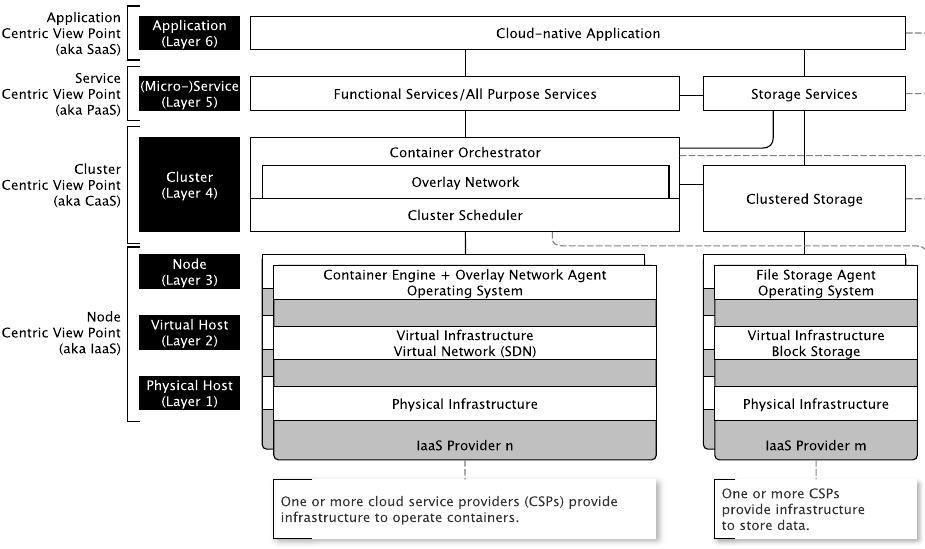
\includegraphics[width=\textwidth]{img/ClouNS_Stack.png}
    \caption[Der ClouNS Stack]{Der ClouNS Stack\cite{kratzke_clouns_2016}}
    \label{fig:clouNS}
\end{figure}

\subsection{Infrastructure as a Service (IaaS)}
Infrastructure as a Service bietet die Grundlage des Cloud Native Stacks. Einem Kunden werden hierbei grundlegende zumeist virtualisierte Hardware-Ressourcen wie Prozessorleistung, Speicher oder Netzwerkmöglichkeiten angeboten. Auf diesen kann er seine Software beliebig ausführen. Er hat dabei keinen Einfluss auf die zugrundeliegende Cloud Infrastruktur (also die Server-Pools an sich), aber kann Betriebssysteme, Anwendungen und verwendeten Speicher kontrollieren\cite{mell_nist_2011}. \\

\subsection{Cluster as a Service (CaaS)}
Bei Cluster as a Service handelt es sich um eine Schicht über IaaS, die ein Clustering von Containern bietet. Hier agieren Orchestrierungs Tools wie zum Beispiel Kubernetes, die Container auf das Cluster verteilen, skalieren und managen\cite{kratzke_clouns_2016}. \\

\subsection{Platform as a Service (PaaS)}
Eine höhere Abstraktionsebene über IaaS oder CaaS. Einem Kunden wird auch hier die Kontrolle über die in der Cloud Infrastruktur auszuführende Anwendung gegeben. Allerdings kann er nicht über verwendete Betriebssysteme, Speichernutzung, Netzwerkkonfiguration usw. entscheiden. Dafür werden ihm vom Anbieter Programmier- oder Laufzeitumgebungen, Tools und Bibliotheken angeboten, die die Entwicklung und Ausführung der Anwendung auf der Infrastruktur ermöglichen\cite{mell_nist_2011}.\\

\subsection{Software as a Service (SaaS)}
Eine höhere Abstraktionsebene über PaaS. Einem Kunden werden hier vom Anbieter explizite auf Cloud Infrastruktur auszuführende Anwendungen bereitgestellt, die dieser verwenden kann. Der Kunde hat weder Einfluss auf die zugrundeliegende Cloud Infrastruktur, noch auf verwendete Betriebssysteme oder Software. Die Ausnahme bilden limitierte Einstellungsmöglichkeiten der vom Anbieter bereitgestellten Anwendung\cite{mell_nist_2011}.

\section{Cloud Native Computing}
Cloud Native Technologien oder Cloud Native Computing ist laut der Cloud Native Computing Foundation (CNCF) eine Ansammlung von Technologien, die es Unternehmen ermöglichen "`skalierbare Anwendungen in modernen, dynamischen Umgebungen zu implementieren und zu betreiben"' \cite{noauthor_cncftoc_nodate}. Bei diesen dynamischen Umgebungen handelt es sich dabei ausschließlich um Cloud Umgebungen (also private, öffentliche und hybride Clouds). Diese Systeme sollen lose gekoppelt, "`belastbar, handhabbar und beobachtbar"' sein und durch Automatisierung schnelle Änderungen ermöglichen\cite{noauthor_cncftoc_nodate}.

\section{Containerisierung}
Containerisierung ist eine Technik, den Code einer Anwendung mitsamt aller Abhängigkeiten, die diese zur Ausführung benötigt, zu verpacken. Ein solches Paket wird als Container Image bezeichnet. Da alle Abhängigkeiten enthalten sind, werden dadurch die Laufzeitunterschiede auf unterschiedlichen Plattformen minimiert\cite{noauthor_what_nodate}. Zur Laufzeit wird ein Container Image als Container bezeichnet. Um ein Container Image auszuführen, wird eine Container Runtime benötigt. Die erste Container Runtime Engine wurde von Docker entwickelt, wird aber mittlerweile als Open-Source Projekt mit dem Namen containerd von der Open Container Initiative (OCI) betrieben\cite{noauthor_what_nodate}. 

Containerisierte Anwendungen unterscheiden sich von Virtuellen Maschinen vor allem darin, dass kein Hypervisor zur Ausführung der Images benötigt wird. Stattdessen teilen sich alle Container das Host-Betriebssystem und werden in einem eigenen User-Space isoliert. Dadurch können Container-Images deutlich leichtgewichtiger und schneller als Virtuelle Maschinen ausgeführt werden. Abbildung \ref{fig:containerVsVMs} verdeutlicht nochmals den Unterschied beider Technologien.

\begin{figure}[H]
    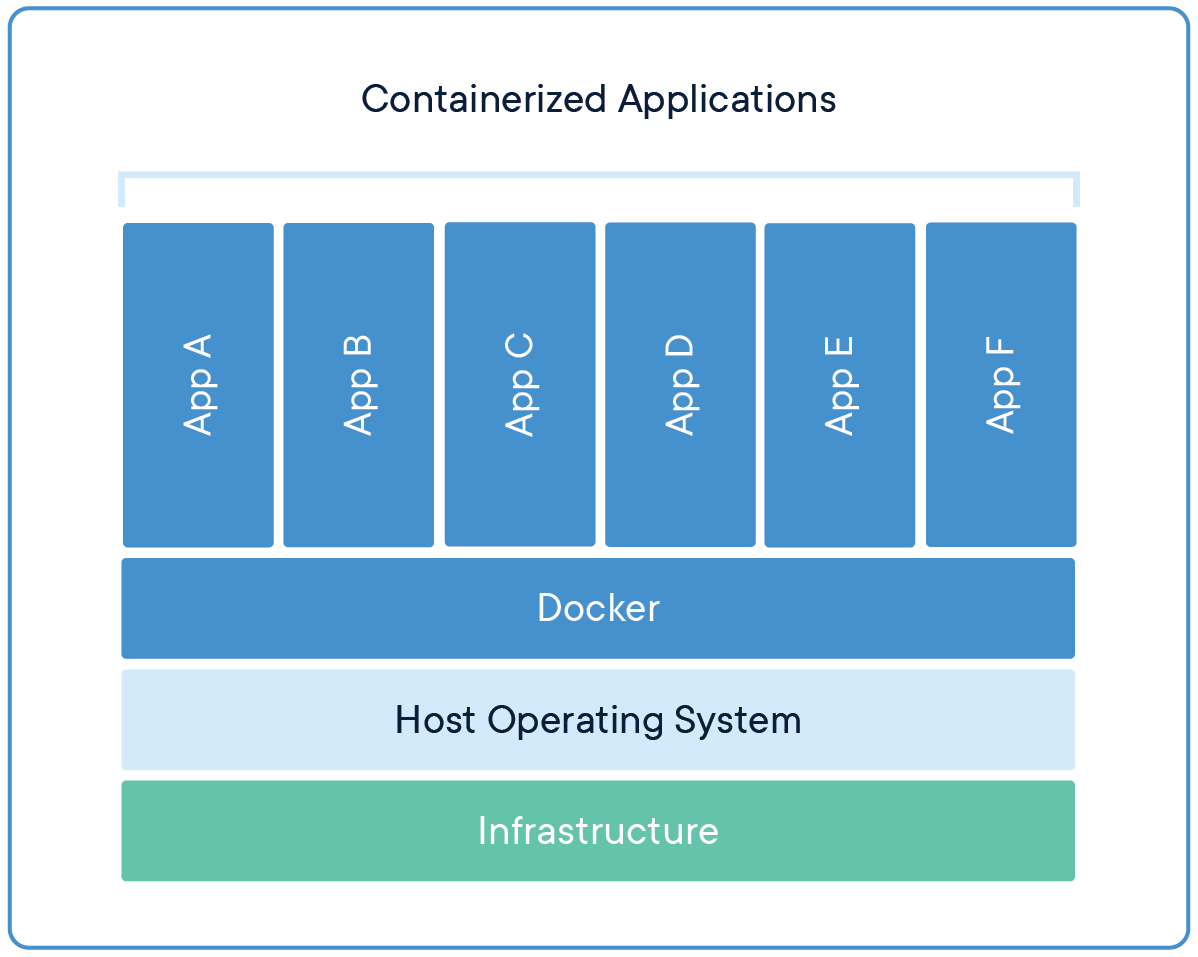
\includegraphics[width=200pt]{img/container-architecture.png}
    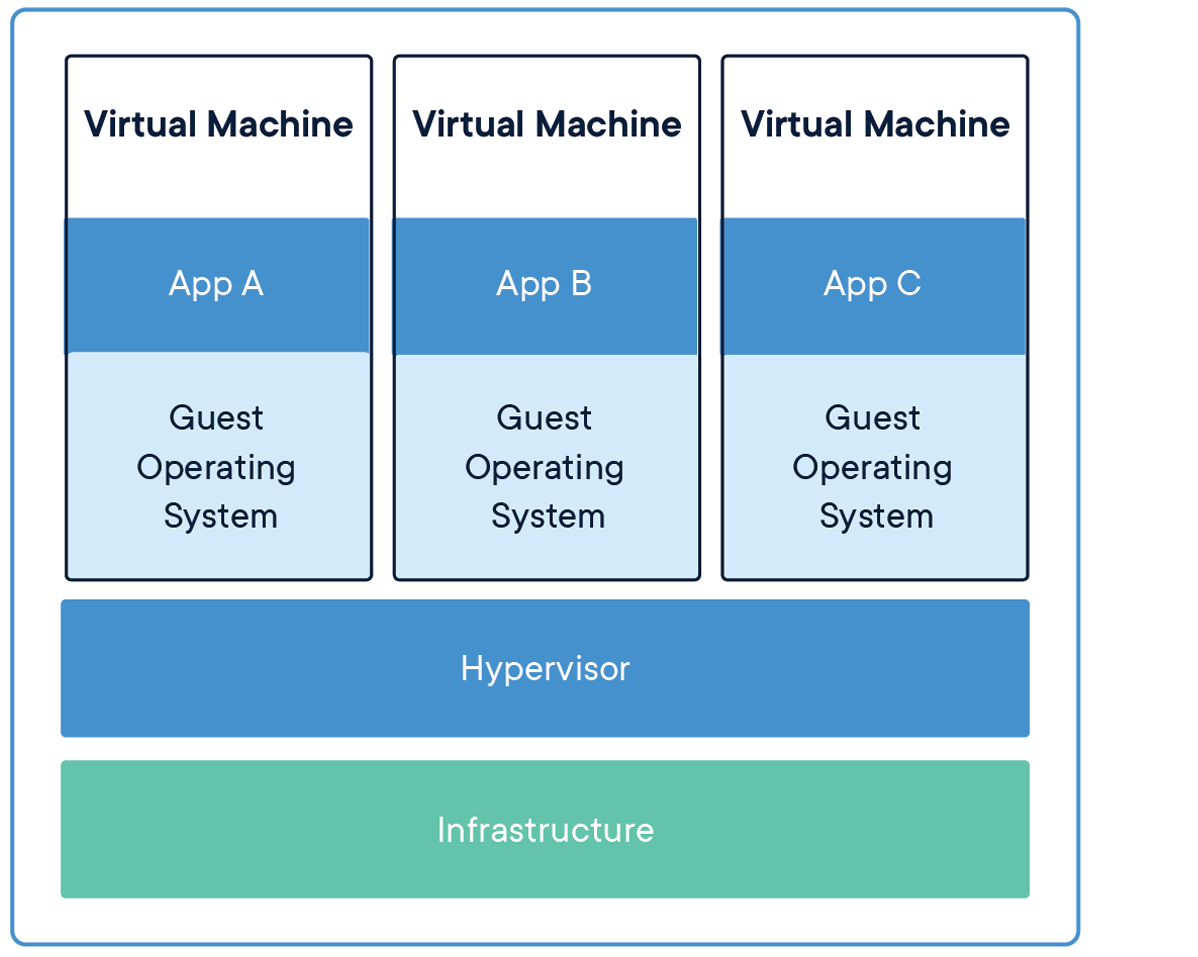
\includegraphics[width=200pt]{img/vm-architecture.png}
    
    \caption[Vergleich zwischen Containern und Virtuellen Maschinen]{Vergleich zwischen Containern und Virtuellen Maschinen\cite{noauthor_what_nodate}}
    \label{fig:containerVsVMs}
\end{figure}

\section{Container-Orchestrierung}
Container-Orchestrierung beschreibt die Automatisierung der "`Bereitstellung, Verwaltung, Skalierung und Vernetzung von Containern"'\cite{noauthor_was_nodate-1}. Mit Orchestrierungs-Tools wie Kubernetes, lassen sich Container einfach auf Computer-Clustern provisionieren, skalieren und überwachen. Wie im ClouNS Modell (Abb. \ref{fig:clouNS}) zu sehen ist, agieren Container Orchestrierungs Tools auf der CaaS Ebene. Dadurch erlauben sie das Betreiben von infrastrukturunabhängigen und flexiblen Anwendungen auf Basis von Containern\cite{noauthor_was_nodate}.

\section{Serverless}
Serverless ist ein Software-Ausführungsmodell, bei dem ein Cloud Anbieter (z.B AWS, Azure, GCP) sich vollständig um die Ausführung einer Anwendung inklusive Konfiguration der zugrundeliegenden Server kümmert. Der Programmierer kann sich daher ausschließlich auf das Schreiben des Codes konzentrieren und muss keine Zeit in das Einstellen und Aufsetzen von Servern investieren. \\
Dabei wird die Software in einem Stateless-Container, d.h einem Container ohne persistentem Speicher, ausgeführt. Der Cloud-Anbieter stellt dabei die Ressourcen dynamisch bzw. on-demand bereit, d.h die Anwendung wird nur dann ausgeführt, wenn eine diesbezügliche Anfrage eintrifft. Serverless verspricht dadurch eine effizientere Entwicklung und Kosteneinsparungen, da bei den Anbietern nur der tatsächlich laufenden Code abgerechnet wird. In der Regel muss vom Entwickler einer Serverless-Anwendung nur eine einzige Funktion geschrieben werden, weshalb Serverless auch als Function-as-a-Service (FaaS) bezeichnet wird\cite{noauthor_was_2016}. \\
Da eine Serverless-Funktion nicht dauerhaft ausgeführt wird, muss bei einem eingetretenen Event erst einmal der Anwendungscontainer aufgesetzt werden. Dies wird als "`Cold Start"' bezeichnet und kann sich als Latenz bei der Ausführung der Funktion bemerkbar machen. Ist der Container einmal gestartet kann er von den Cloud-Anbietern vorgehalten werden und bei der nächsten Anfrage schneller reagieren. Dies wird auch als "`Warm Start"' bezeichnet\cite{noauthor_was_2016}. Es gibt einige Techniken, um seine Funktionen möglichst warm zu halten, die auch in dieser Arbeit untersucht werden.